\documentclass[]{article}
\usepackage{tikz}
\usepackage{tikz,fullpage}
\usetikzlibrary{arrows,%
	petri,%
	topaths}%
\usepackage{tkz-berge}
\usepackage[position=top]{subfig}
\usepackage{amsmath}
\usepackage{amsfonts}
\usepackage{amssymb}
\usepackage{graphicx}
\usepackage{textcomp}
\usepackage{logicproof}
\usepackage{tabularx}
\usepackage{float}
%opening
\title{Bioinformatics Summative Assignment 2018-19}
\author{clvp22} %REPLACE WITH YOUR CIS CODE

\begin{document}

\maketitle


\section{Question 2}
\begin{enumerate}
\item We begin with the following distance matrix,
\begin{center}
\begin{tabular}{|c|c|c|c|c|c|c|}
	\hline
	& a & b & c & d & e & f \\
	\hline
	a & 0 & 15 & 24 & 29 & 25 & 37 \\
	\hline
	b & 15 & 0 & 32 & 31 & 23 & 43 \\
	\hline
	c & 24 & 32 & 0 & 30 & 43 & 49 \\
	\hline
	d & 29 & 31 & 30 & 0 & 45 & 57 \\
	\hline
	e & 25 & 23 & 43 & 45 &0 & 55 \\
	\hline
	f & 37 & 43& 49 & 57 & 55 & 0 \\
	\hline
\end{tabular}
\end{center}
\item Clearly species \textit{a} and \textit{b} are the closest pair of species so we cluster these species together to get a new species \textit{ab} and the following matrix,
\begin{center}
\begin{tabular}{|c|c|c|c|c|c|}
	\hline
	& ab & c & d & e & f \\
	\hline
	ab & 0 & 28 & 30 & 24 & 40 \\
	\hline
	c & 28 & 0 & 30 & 43 & 49 \\
	\hline
	d & 30 & 30 & 0 & 45 & 57 \\
	\hline
	e & 24 & 43 & 45 &0 & 55 \\
	\hline
	f & 40& 49 & 57 & 55 & 0 \\
	\hline
\end{tabular}
\end{center}
\item We can begin to construct our phylogenetic tree as follows,
\begin{figure}[H]
	\begin{center}
		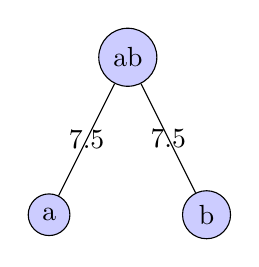
\begin{tikzpicture}[main_node/.style={circle,fill=blue!20,draw,minimum size=1em,inner sep=3pt]}]

		\node[main_node] (1) at (0,0) {a};
		\node[main_node] (2) at (2,0) {b};
		\node[main_node] (3) at (1,2) {ab};


		\draw (1) edge node{7.5} (3);
		\draw (2) edge node{7.5} (3);
		\end{tikzpicture}
	\end{center}
	\caption{Phlyogenetic Tree}
	\label{Phlyogenetic Tree}
\end{figure}
\newpage
\item Now species \textit{ab} and \textit{e} are the closest pair of species in our matrix so we reduce the matrix by creating a new cluster of species \textit{abe}. Because we are following the UPGMA algorithm we must use the following formula to calculate the distances, $$d(abe,x) = \frac{2 \cdot d(ab,x) + 1 \cdot d(e,x)}{2+1} $$ for some \textit{x}.
\\
\\
Consequently we get the following matrix,
\begin{center}
\begin{tabular}{|c|c|c|c|c|}
	\hline
	& abe & c & d & f \\
	\hline
	abe & 0 & 33 & 35 & 45 \\
	\hline
	c & 33 & 0 & 30 & 49 \\
	\hline
	d & 35 & 30 & 0 & 57 \\
	\hline
	f & 45& 49 & 57 & 0 \\
	\hline
\end{tabular}
\end{center}
\item We continue to build our phylogenetic tree,
\begin{figure}[H]
	\begin{center}
		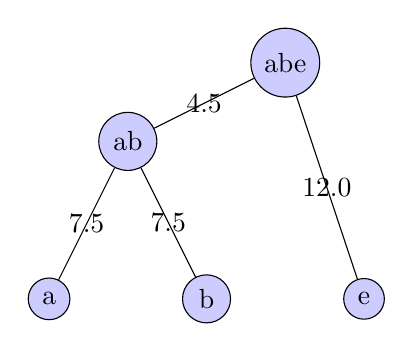
\begin{tikzpicture}[main_node/.style={circle,fill=blue!20,draw,minimum size=1em,inner sep=3pt]}]

		\node[main_node] (1) at (0,0) {a};
		\node[main_node] (2) at (2,0) {b};
		\node[main_node] (3) at (1,2) {ab};
		\node[main_node] (4) at (4,0) {e};
		\node[main_node] (5) at (3,3) {abe};


		\draw (1) edge node{7.5} (3);
		\draw (2) edge node{7.5} (3);
		\draw (3) edge node{4.5} (5);
		\draw (4) edge node{12.0} (5);
		\end{tikzpicture}
	\end{center}
	\caption{Phlyogenetic Tree}
	\label{Phlyogenetic Tree}
\end{figure}
\item We reduce our matrix again by clustering the new closest pair of species \textit{c} and \textit{d} into \textit{cd} to get the following matrix,
\begin{center}
\begin{tabular}{|c|c|c|c|}
	\hline
	& abe & cd & f \\
	\hline
	abe & 0 & 34 & 45 \\
	\hline
	cd & 34 & 0 & 53 \\
	\hline
	f & 45& 53 & 0 \\
	\hline
\end{tabular}
\end{center}
\item We continue to build our phylogenetic tree,
\begin{figure}[H]
	\begin{center}
		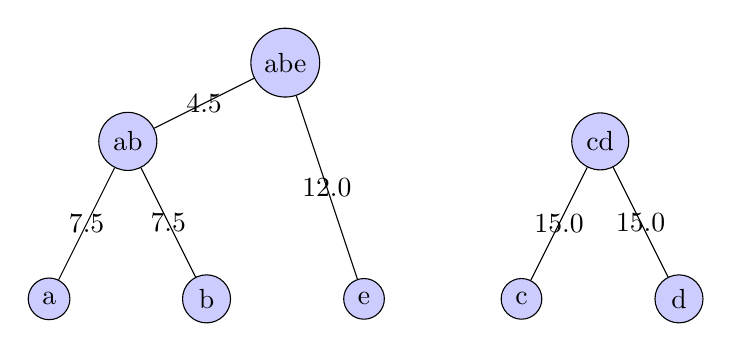
\begin{tikzpicture}[main_node/.style={circle,fill=blue!20,draw,minimum size=1em,inner sep=3pt]}]

		\node[main_node] (1) at (0,0) {a};
		\node[main_node] (2) at (2,0) {b};
		\node[main_node] (3) at (1,2) {ab};
		\node[main_node] (4) at (4,0) {e};
		\node[main_node] (5) at (3,3) {abe};
		\node[main_node] (6) at (6,0) {c};
		\node[main_node] (7) at (8,0) {d};
		\node[main_node] (8) at (7,2) {cd};

		\draw (1) edge node{7.5} (3);
		\draw (2) edge node{7.5} (3);
		\draw (3) edge node{4.5} (5);
		\draw (4) edge node{12.0} (5);
		\draw (6) edge node{15.0} (8);
		\draw (7) edge node{15.0} (8);
		\end{tikzpicture}
	\end{center}
	\caption{Phlyogenetic Tree}
	\label{Phlyogenetic Tree}
\end{figure}
\item We now reduce our matrix by clustering the clusters \textit{abe} and \textit{cd}, again we are following the UPGMA algorithm so, $$d(abecd,f) = \frac{3 \cdot d(abe,f) + 2 \cdot d(cd,f)}{3+2} $$. We get the following matrix,
\begin{center}
\begin{tabular}{|c|c|c|}
	\hline
	& abecd & f \\
	\hline
	abecd & 0 & 48.2 \\
	\hline
	f & 48.2&  0 \\
	\hline
\end{tabular}
\end{center}
\item We continue to build our phylogenetic tree,
\begin{figure}[H]
	\begin{center}
		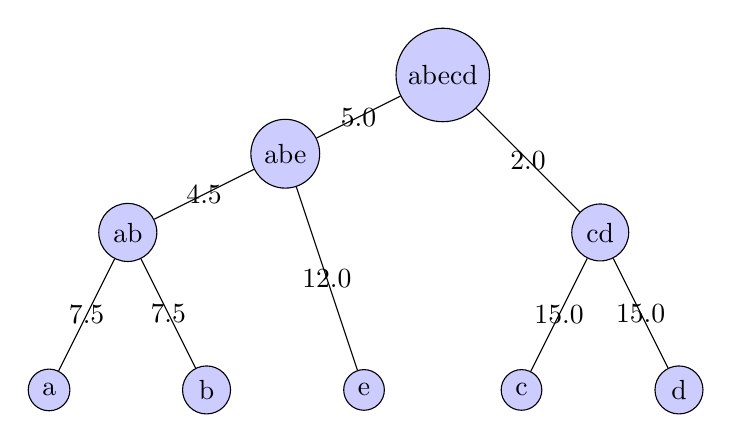
\begin{tikzpicture}[main_node/.style={circle,fill=blue!20,draw,minimum size=1em,inner sep=3pt]}]

		\node[main_node] (1) at (0,0) {a};
		\node[main_node] (2) at (2,0) {b};
		\node[main_node] (3) at (1,2) {ab};
		\node[main_node] (4) at (4,0) {e};
		\node[main_node] (5) at (3,3) {abe};
		\node[main_node] (6) at (6,0) {c};
		\node[main_node] (7) at (8,0) {d};
		\node[main_node] (8) at (7,2) {cd};
		\node[main_node] (9) at (5,4) {abecd};

		\draw (1) edge node{7.5} (3);
		\draw (2) edge node{7.5} (3);
		\draw (3) edge node{4.5} (5);
		\draw (4) edge node{12.0} (5);
		\draw (6) edge node{15.0} (8);
		\draw (7) edge node{15.0} (8);
		\draw (5) edge node{5.0} (9);
		\draw (8) edge node{2.0} (9);
		\end{tikzpicture}
	\end{center}
	\caption{Phlyogenetic Tree}
	\label{Phlyogenetic Tree}
\end{figure}
\item Finally, we need not reduce our matrix any further, because we can simply add our remaining species \textit{f} to the phylogenetric tree as follows to get our solution,
\begin{figure}[H]
	\begin{center}
		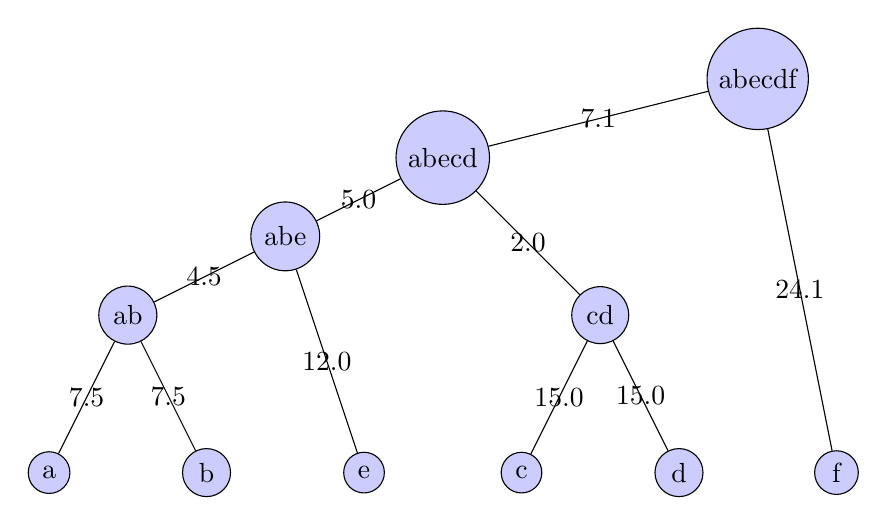
\begin{tikzpicture}[main_node/.style={circle,fill=blue!20,draw,minimum size=1em,inner sep=3pt]}]

		\node[main_node] (1) at (0,0) {a};
		\node[main_node] (2) at (2,0) {b};
		\node[main_node] (3) at (1,2) {ab};
		\node[main_node] (4) at (4,0) {e};
		\node[main_node] (5) at (3,3) {abe};
		\node[main_node] (6) at (6,0) {c};
		\node[main_node] (7) at (8,0) {d};
		\node[main_node] (8) at (7,2) {cd};
		\node[main_node] (9) at (5,4) {abecd};
		\node[main_node] (10) at (10,0) {f};
		\node[main_node] (11) at (9,5) {abecdf};

		\draw (1) edge node{7.5} (3);
		\draw (2) edge node{7.5} (3);
		\draw (3) edge node{4.5} (5);
		\draw (4) edge node{12.0} (5);
		\draw (6) edge node{15.0} (8);
		\draw (7) edge node{15.0} (8);
		\draw (5) edge node{5.0} (9);
		\draw (8) edge node{2.0} (9);
		\draw (9) edge node{7.1} (11);
		\draw (10) edge node{24.1} (11);
		\end{tikzpicture}
	\end{center}
	\caption{Final Phlyogenetic Tree}
	\label{Final Phlyogenetic Tree}
\end{figure}
\end{enumerate}


\end{document}